\documentclass[12pt]{article}

\usepackage[spanish]{babel}
\usepackage[none]{hyphenat}
\usepackage{enumitem}
\usepackage{listings}
\usepackage{color}
\usepackage[hidelinks]{hyperref}
\usepackage{graphicx}
\usepackage[export]{adjustbox}

\definecolor{dkgreen}{rgb}{0,0.6,0}
\definecolor{gray}{rgb}{0.5,0.5,0.5}
\definecolor{mauve}{rgb}{0.58,0,0.82}

\lstset{
    language=Java,
    aboveskip=3mm,
    belowskip=3mm,
    showstringspaces=false,
    columns=flexible,
    basicstyle={\tiny\ttfamily},
    numbers=none,
    numberstyle=\tiny\color{gray},
    keywordstyle=\color{blue},
    commentstyle=\color{dkgreen},
    stringstyle=\color{mauve},
    breaklines=true,
    breakatwhitespace=true,
    tabsize=3
}

\sloppy
\setlength{\parindent}{0cm}
\decimalpoint
\setenumerate[2]{label=\alph*)}
\hypersetup{colorlinks=true, urlcolor=blue, citecolor=blue}
\urlstyle{same}
\newcommand{\linejump}{\hfill \break}
\graphicspath{{img/}}

\begin{document}
    \begin{center}
        \large \textbf{Operadores lógicos y Operador Ternario}
    \end{center}
    
    \begin{flushright}
        32020610-2. \\
        Acosta Porcayo Alan Omar.
    \end{flushright}

    \begin{enumerate}[leftmargin=*]
        \item Investigue los siguientes conceptos relacionados a POO y describa con sus propias palabras la definición de cada uno de ellos:
        \begin{enumerate}[leftmargin=*]
            \item Modularidad: es una forma de escribir código en la que un programa se divide en múltiples entidades que realizan una tarea especifica y solo se comunican entre ellas para intercambiar información.
            \item Jerarquía de clases: se basa en la relación de la herencia de atributos y métodos de una clase base a otras clases derivadas.
            \item Casting (Moldeado) de tipos primitivos de Java: es el cambio del tipo de una variable. En java solo se puede realizar entre tipos \textit{int, long, float, double} y \textit{char}.
            \item Diferencia entre referencia y objeto: una referencia es la dirección de memoria en que se guarda una variable u objeto, en cambio un objeto es la instanciación de una clase.
            \item Uso de las palabras reservadas \textit{new}, \textit{finalize} y \textit{this}: \textit{new} se utiliza para crear una instancia de un clase, es decir un objeto. \textit{finalize} sirve para eliminar un objeto. \textit{this} se usa para hacer una referencia al objeto actual e invocar un constructor de la clase instanciada. 
        \end{enumerate}

        \newpage
        \item Sea $a = 11 , b = 33$ y $c = 3$ Realice las siguientes operaciones lógicas a mano.
        \begin{itemize}[leftmargin=*]
            \item $a$ \& $b$ \& $c = 1$
            \item $a$ $\mid$ $b$ \& $b = 43$ 
            \item $a$ $^{\wedge}$ $c$ $^{\wedge}$ $b = 41$
            \item $a$ $\mid$ $c$ $^{\wedge}$ $b$ $\&$ $c = 10 $
        \end{itemize}
        \begin{figure*}[ht]
            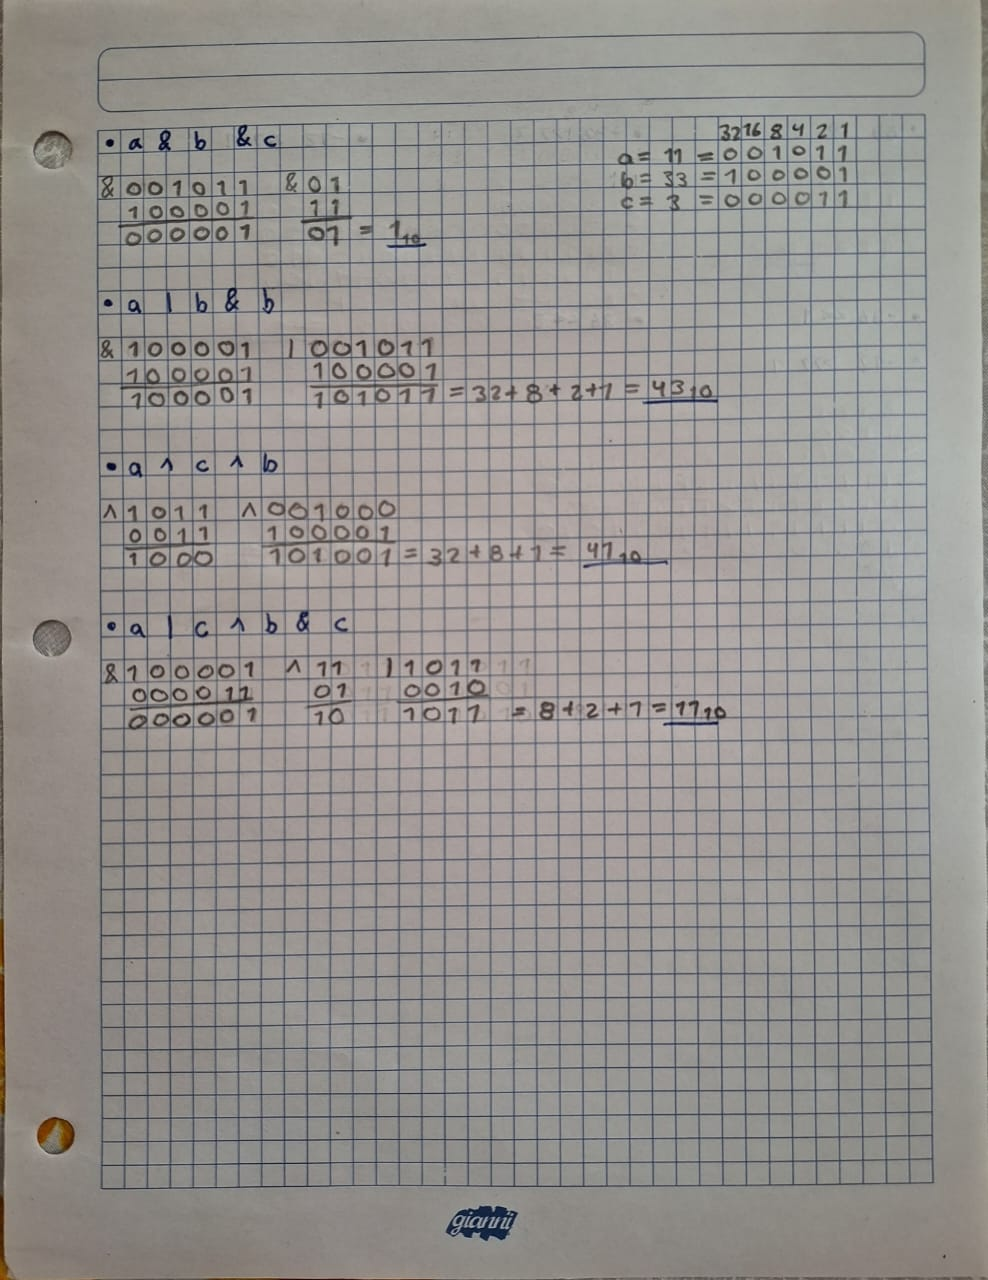
\includegraphics[width = 10cm, center]{E2.jpg}
        \end{figure*}

        \newpage
        \item Investigue el deslizamiento $\gg$, $\ll$, $\gg>$ y realice las siguientes operaciones a mano:
        \begin{itemize}[leftmargin=*]
            \item $13 \gg 2 = 3$
            \item $-36 \gg 3 = -5$
            \item $-12 \gg> 1 = -32762$
            \item $-36 \ll 1 = -72$ 
            \item $36 \ll 2 = 144$
        \end{itemize}
        \begin{figure*}[ht]
            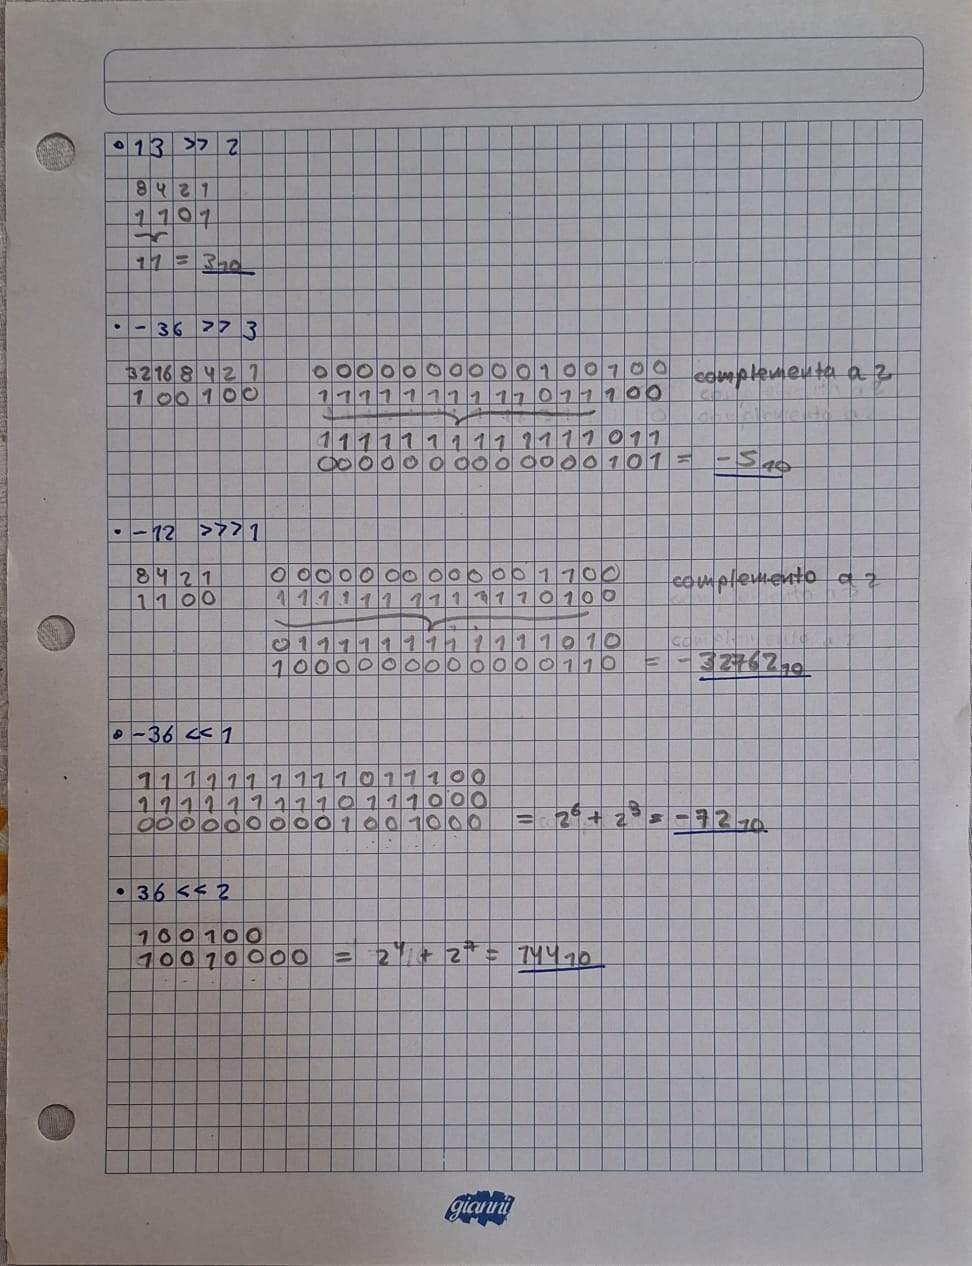
\includegraphics[width = 10cm, center]{E3.jpg} 
        \end{figure*}
        \newpage

        Después de realizar las operaciones de deslizamientos a la izquierda y a la derecha a ¿qué tipo de operaciones aritméticas serian equivalentes?

        Con multiplicaciones y divisiones enteras por dos.

        Para realizar dichas operaciones utilice el complemento a 2 de un número binario en el caso de que el número entero sea negativo y considere que un \textbf{int} es de 16 bits en java.

        \item Modifique el programa Adivina.java y agregue donde sea posible el operador ternario de java.
        \begin{lstlisting}
import java.util.Scanner;
import java.util.Random;

public class Adivina {
    public static void main(String[] args) {
        Scanner s = new Scanner(System.in);
        Random t = new Random();

        int i = 4, a = t.nextInt(100);

        while (i > 0) {
            System.out.print("Adivina el numero entre 0-99 : ");
            int b = s.nextInt();
            i--;

            if (a == b)
                break;
            else if (i != 0){
                System.out.println("Un intento menos");
                System.out.println(a > b ? "Mas\n" : "Menos\n");
            }
        }
        s.close();

        System.out.println(i == 0 ? "\nNo pudiste! El numero aleatorio es: " + a : "\nLe atinaste al numero aleatorio");
    }
}   
        \end{lstlisting}
    \end{enumerate}

    \subsection*{Referencias Bibliográficas}
    IBM Documentation. (2023, March 23). \url{https://www.ibm.com/docs/es/aix/7.3?topic=processes-modularity}

    \linejump
    Tyflos. (2022, May 6). \textit{Jerarquías de clase dentro de la Programación orientada a objetos.} Programar a Ciegas. \url{https://programaraciegas.net/?p=889}

    \linejump
    bloque2:casting [\textit{Programación}]. (n.d.). \url{https://programacion.abrilcode.com/doku.php?id=bloque2:casting}

    \linejump
    Miraladiferencia. (2020, December 28). \textit{Diferencia entre referencia y objeto en Java (con tabla)} \url{https://miraladiferencia.com/it/diferencia-entre-referencia-y-objeto-en-java-con-tabla/}

    \linejump
    \textit{Palabras clave (reservadas) del lenguaje Java.} (n.d.). Abrirllave.com. https://www.abrirllave.com/java/palabras-clave.php

    \linejump
    GeeksforGeeks. (2022). Shift Operator in Java. \textit{GeeksforGeeks.} \url{https://www.geeksforgeeks.org/shift-operator-in-java/}
\end{document}
